\documentclass[12pt]{beamer}
\usepackage{../Estilos/BeamerFC}
\usepackage{../Estilos/ColoresLatex}
\input{../Preambulos/pre_codigo}
\input{../Preambulos/preambulo_Beamer_Warsaw_seahorse}
%\usefonttheme{serif}

\title{\large{Tema 1 - Errores y artimética de punto flotante}}
\author{M. en C. Gustavo Contreras Mayén}
\date{ }

\begin{document}
\maketitle

\section*{Contenido}
\frame[allowframebreaks]{\frametitle{Contenido} \tableofcontents[currentsection, hideallsubsections]}

\section{Tema 1}
\frame[allowframebreaks]{\frametitle{Contenido} \tableofcontents[currentsection, hideothersubsections]}
\subsection{Objetivos del Tema}

\begin{frame}
\frametitle{Objetivos}
Al concluir el Tema 1, el alumno:
\setbeamercolor{item projected}{bg=lava,fg=white}
\setbeamertemplate{enumerate items}{%
\usebeamercolor[bg]{item projected}%
\raisebox{1.5pt}{\colorbox{bg}{\color{fg}\footnotesize\insertenumlabel}}%
}
\begin{enumerate}[<+->]
\item Reconocerá la diferencia entre \textocolor{ao}{error absoluto} y \textocolor{carmine}{error relativo}.
\item Diferenciará los conceptos de: \textocolor{byzantine}{precisión}, \pause \textocolor{cadmiumgreen}{exactitud}, \pause \textocolor{cadmiumred}{condición}, \pause \textocolor{cobalt}{estabilidad} \pause y \textocolor{bole}{eficiencia}.
\seti
\end{enumerate}
\end{frame}
\begin{frame}
\frametitle{Objetivos}
\setbeamercolor{item projected}{bg=lava,fg=white}
\setbeamertemplate{enumerate items}{%
\usebeamercolor[bg]{item projected}%
\raisebox{1.5pt}{\colorbox{bg}{\color{fg}\footnotesize\insertenumlabel}}%
}
\begin{enumerate}[<+->]
\conti
\item Reconocerá la representación de punto flotante para el manejo de números en una computadora.
\end{enumerate}
\end{frame}

\section{Física Computacional}
\frame[allowframebreaks]{\frametitle{Contenido}  \tableofcontents[currentsection, hideothersubsections]}
\subsection{¿Qué es la FC?}

\begin{frame}
\frametitle{La física antes de la era computacional}
Antes del desarrollo y \enquote{boom} computacional, la física presentaba dos grandes áreas:
\pause
\begin{figure}
	\centering
	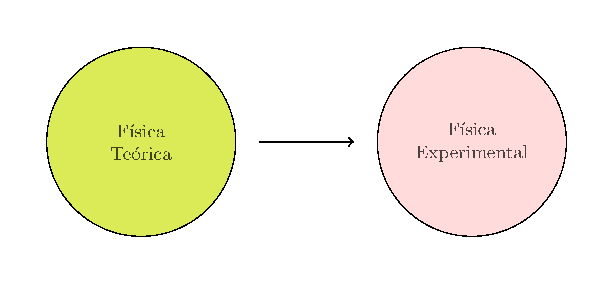
\includegraphics[scale=1]{Imagenes/figura_02.eps}
	\end{figure}
\end{frame}
\begin{frame}
\frametitle{¿Qué es la física computacional?}
La física computacional es una nueva manera de hacer investigación en física, próxima al
experimento y a la teoría.
\\
\bigskip
\pause
En el laboratorio se realizan mediciones en sistemas físicos reales (restringida a la factibilidad de recursos técnicos), y que luego los físicos teóricos explican esas mediciones mediante las teorías.
\end{frame}
\begin{frame}[fragile]
\frametitle{El proceso de trabajo}
\begin{figure}
	\centering
	\hspace*{-1cm}
	\includegraphics[scale=0.7]{Imagenes/figura_03.eps}
\end{figure}
\end{frame}
\begin{frame}[fragile]
\frametitle{Interesección de varias áreas}
\begin{figure}
	\centering
	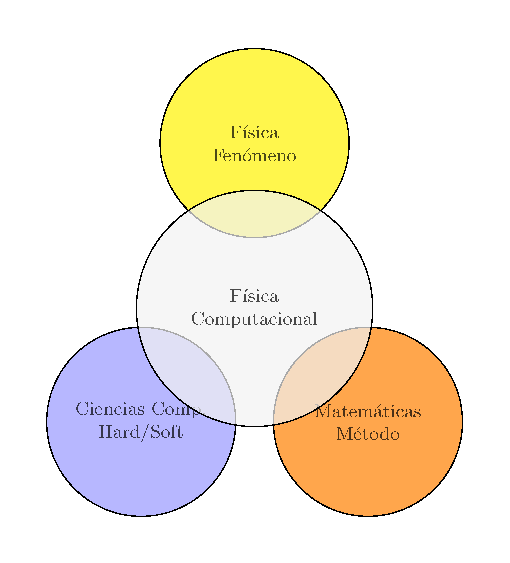
\includegraphics[scale=0.7]{Imagenes/figura_01.eps}
\end{figure}
\end{frame}
\begin{frame}[fragile]
\frametitle{La física computacional}
Con la incorporación de una herramienta tan poderosa como es la computación, la física como ciencia, cuenta ahora con una extensión en su estudio.
\\
\bigskip
\pause
De manera general se entiende que la física computacional tiene lo siguiente:
\end{frame}
\begin{frame}[fragile]
\begin{figure}
	\centering
	\includegraphics[scale=0.8]{Imagenes/figura_04.eps}
\end{figure}
\end{frame}
\begin{frame}
\frametitle{Áreas de investigación en la física}
\begin{itemize}[<+->]
	\item[\ding{51}] Problemas que no tienen solución analítica.
	\item[\ding{51}] Validar aproximaciones y hacer efectivas las teorías propuestas.
	\item[\ding{51}] Comparar cuantitativamente teorías y mediciones experimentales.
	\item[\ding{51}] Visualizar conjuntos de datos complejos.
	\item[\ding{51}] Control y medición de experimentos.
\end{itemize}
\end{frame}
\begin{frame}
\frametitle{Campos para la física computacional}
\begin{multicols}{2}
\begin{itemize}[<+->]
\item[\ding{213}] Predicción del clima
\item[\ding{213}] Superconductividad
\item[\ding{213}] Genoma Humano
\item[\ding{213}] Visión y lenguaje
\item[\ding{213}] Fusión nuclear
\item[\ding{213}] Oceanografía
\item[\ding{213}] Ciencia de los materiales
\item[\ding{213}] Diseño de semiconductores
\item[\ding{213}] Astrofísica relativista
\end{itemize}
\end{multicols}
\end{frame}
\begin{frame}
\frametitle{Campos para la física computacional}
\begin{multicols}{2}
\begin{itemize}[<+->]
\item[\ding{213}] Sistemas de combustión
\item[\ding{213}] Estructura biológica
\item[\ding{213}] Diseño de fármacos
\item[\ding{213}] Turbulencia
\item[\ding{213}] Recuperación de petróleo y gas
\item[\ding{213}] Cromodinámica cuántica
\end{itemize}
\end{multicols}
\end{frame}
\begin{frame}
\frametitle{Alcance del curso}
El curso está diseñado para ofrecer una introducción a los métodos numéricos aplicados a la física.
\\
\bigskip
\pause
Se dará un punto de referencia para continuar profundizando de manera particular en temas específicos. 
\end{frame}
\begin{frame}
\frametitle{Alcance del curso}
El desarrollo de las habilidades de programación, están en función del tiempo dedicado al trabajo fuera de la clase, pero consideramos que se abren un panorama diferente para abordar ya sea un servicio social, tesis o proyecto de trabajo para un posgrado.
\end{frame}
\begin{frame}[fragile]
\frametitle{Animación básica con \python}
\begin{center}
\movie[externalviewer]{
    \includegraphics[width=0.5\textheight, keepaspectratio]{Imagenes/video_icon.png}}{animacion_basica.mp4}
\end{center}
\end{frame}
\begin{frame}[fragile]
\frametitle{Animación de un péndulo doble}
\begin{center}
\movie[externalviewer, width=5.25cm, height=4cm, autostart, loop]{
    \includegraphics[width=0.5\textheight, keepaspectratio]{Imagenes/video_icon.png}}{double_pendulum.mp4}
\end{center}
\end{frame}

\section{Computadoras y números}
\frame[allowframebreaks]{\frametitle{Contenido} \tableofcontents[currentsection, hideothersubsections]}
\subsection{Conceptos básicos}

\begin{frame}
\frametitle{Nuestra experiencias usando una computadora}
El uso de una computadora es algo tan común para nosotros hoy en día.
\\
\bigskip
\pause
Así como otros dispositivos como: tabletas, celulares, smart tv, etc.
\end{frame}
\begin{frame}
\frametitle{Usando una computadora}
En algún momento hemos trabajado con:
\setbeamercolor{item projected}{bg=black,fg=white}
\setbeamertemplate{enumerate items}{%
\usebeamercolor[bg]{item projected}%
\raisebox{1.5pt}{\colorbox{bg}{\color{fg}\footnotesize\insertenumlabel}}%
}
\begin{enumerate}[<+->]
\item Procesador de textos.
\item Hoja de cálculo.
\item Presentaciones.
\end{enumerate}
\end{frame}
\begin{frame}
\frametitle{Usando una computadora}
Además de:
\setbeamercolor{item projected}{bg=airforceblue,fg=aliceblue}
\setbeamertemplate{enumerate items}{%
\usebeamercolor[bg]{item projected}%
\raisebox{1.5pt}{\colorbox{bg}{\color{fg}\footnotesize\insertenumlabel}}%
}
\begin{enumerate}[<+->]
\item Ver videos.
\item Streaming.
\item Redes sociales.
\item Etc.
\end{enumerate}
\end{frame}
\begin{frame}
\frametitle{Primera impresión con el uso de computadoras}
Al usar una computadora nos damos cuenta de que ésta hace lo que le pedimos.
\\
\bigskip
\pause
En una primera impresión \enquote{entendemos} que no hay errores en la ejecución de las tareas en la computadora. \pause Esa impresión va a cambiar en unos momentos.
\end{frame}
\begin{frame}[fragile]
\frametitle{Realiza la siguiente operación}
En una notebook de Jupyter, escribe la siguiente operación:
\begin{lstlisting}[caption=Diferencia entre dos valores]
1.1 - 0.1
\end{lstlisting}
\pause
\textbf{¿Qué pasó con el resultado?}
\end{frame}
\begin{frame}
\frametitle{Errores durante el proceso de cálculo}
\setbeamercolor{item projected}{bg=arsenic,fg=aureolin}
\setbeamertemplate{enumerate items}{%
\usebeamercolor[bg]{item projected}%
\raisebox{1.5pt}{\colorbox{bg}{\color{fg}\footnotesize\insertenumlabel}}%
}
\begin{enumerate}[<+->]
\item Como usuarios ingresamos un número exacto $x$, que generalmente está en base $10$.
\item La computadora almacena $x$ en su formato interno, lo redondea si no puede representarlo de manera exacta, ocupando base $2$.
\item El valor inicial $x$ pasa a ser $x + \delta$. \pause Esperamos que el valor de $\delta$ sea pequeño.
\seti
\end{enumerate}
\end{frame}
\begin{frame}
\frametitle{Errores durante el proceso de cálculo}
\setbeamercolor{item projected}{bg=arsenic,fg=aureolin}
\setbeamertemplate{enumerate items}{%
\usebeamercolor[bg]{item projected}%
\raisebox{1.5pt}{\colorbox{bg}{\color{fg}\footnotesize\insertenumlabel}}%
}
\begin{enumerate}[<+->]
\conti
\item La computadora realiza operaciones con $x + \delta$ y obtiene el resultado $f (x + \delta)$.
\item Se convierte el valor de $f (x + \delta)$ del formato interno a la salida que el usuario lee, en caso de ser necesario la computadora redondea el valor.
\item Como usuarios leemos el resultado $f (x + \delta) + \varepsilon$, debido al redondeo durante la conversión.
\end{enumerate}
\end{frame}
\begin{frame}
\frametitle{Consideración importante}
En algunos casos, la representación del valor $x$ puede ser exacta.
\\
\bigskip
\pause
En general, los errores se presentan cuando manejamos números fraccionarios, donde es común que no exista la representación exacta en la computadora.
\end{frame}
\begin{frame}
\frametitle{Estudiando las fuentes de error}
Es importante que comprendamos desde el inicio del curso las fuentes del error.
\\
\bigskip
\pause
Para que en la solución numérica de problemas se tenga el valor más pequeño de ese error.
\end{frame}

\section{Errores}
\frame[allowframebreaks]{\frametitle{Contenido} \tableofcontents[currentsection, hideothersubsections]}
\subsection{Calculando errores}

\begin{frame}
\frametitle{Valor exacto y aproximado}
En el cálculo numérico con el uso de expresiones artiméticas encontraremos que:
\setbeamercolor{item projected}{bg=ballblue,fg=beige}
\setbeamertemplate{enumerate items}{%
\usebeamercolor[bg]{item projected}%
\raisebox{1.5pt}{\colorbox{bg}{\color{fg}\footnotesize\insertenumlabel}}%
}
\begin{enumerate}[<+->]
\item Son pocos los casos en donde tendremos un resultado exacto.
\item En los otros se buscará una aproximación paulatina al valor exacto.
\item Haremos un alto cuando encontramos que la aproximación no mejora aunque no lleguemos al valor exacto.
\end{enumerate}
\end{frame}
\begin{frame}
\frametitle{Pregunta inmediata}
La pregunta que debemos de responder con un sustento científico y no por apreciación es:
\pause
\begin{center}
    \textocolor{blue}{¿Que tan pequeña debe de ser una diferencia mínima?}
\end{center}
\end{frame}
\begin{frame}
\frametitle{Definiendo dos tipos de error}
Para dar ese sustento a la respuesta, debemos de considerar dos tipos de error:
\setbeamercolor{item projected}{bg=blue,fg=blond}
\setbeamertemplate{enumerate items}{%
\usebeamercolor[bg]{item projected}%
\raisebox{1.5pt}{\colorbox{bg}{\color{fg}\footnotesize\insertenumlabel}}%
}
\begin{enumerate}[<+->]
\item Error absoluto.
\item Error relativo.
\end{enumerate}
\end{frame}

\subsection{Error absoluto}

\begin{frame}
\frametitle{Definición de valor absoluto}
Hagamos que $x^{*}$ sea la aproximación que tenemos, mientras que $x$ es el valor exacto.
\\
\bigskip
\pause
El error absoluto se define como:
\begin{align*}
E_{\text{abs}} = \abs{ \, x - x^{*}}
\end{align*}
\end{frame}
\begin{frame}
\frametitle{Entendiendo el error absoluto}
Revisemos el siguiente ejemplo:
\setbeamercolor{item projected}{bg=blue-violet,fg=bisque}
\setbeamertemplate{enumerate items}{%
\usebeamercolor[bg]{item projected}%
\raisebox{1.5pt}{\colorbox{bg}{\color{fg}\footnotesize\insertenumlabel}}%
}
\begin{enumerate}[<+->]
\item Si se aproxima $x = 100$ con $x^{*} = 99$ \pause $\to E_{\text{abs}} = 1$ \pause
\item Si se aproxima $x = 1000$ con $x^{*} = 999$ \pause $\to E_{\text{abs}} = 1$
\end{enumerate}
\pause
El error absoluto \textocolor{awesome}{no nos indica la magnitud} del problema que tenemos que aproximar. \pause Debemos de ser cuidadosos reportando este tipo de error.
\end{frame}

\subsection{Error relativo}

\begin{frame}
\frametitle{Definiendo al error relativo}
Para calcular la magnitud del error, ocupemos la siguiente expresión:
\pause
\begin{align*}
E_{\text{rel}} = \abs{\dfrac{x - x^{*}}{x}}
\end{align*}
que nos define el \textocolor{blue-violet}{error relativo}. \pause Cuando se multiplica por 100, tendremos ahora un porcentaje del error.
\end{frame}
\begin{frame}
\frametitle{Del ejemplo anterior}
Expresando el error relativo tendremos que:
\pause
\setbeamercolor{item projected}{bg=blue-violet,fg=bisque}
\setbeamertemplate{enumerate items}{%
\usebeamercolor[bg]{item projected}%
\raisebox{1.5pt}{\colorbox{bg}{\color{fg}\footnotesize\insertenumlabel}}%
}
\begin{enumerate}[<+->]
\item Si se aproxima $x = 100$ con $x^{*} = 99$ \pause $\to E_{\text{rel}} = 1\%$ \pause
\item Si se aproxima $x = 1000$ con $x^{*} = 999$ \pause $\to E_{\text{abs}} = 0.1\%$
\end{enumerate}
\end{frame}    
\begin{frame}
\frametitle{Rango de valores para el error relativo}
El rango para el error relativo se maneja entre dos valores:
\pause
\setbeamercolor{item projected}{bg=bole,fg=brightgreen}
\setbeamertemplate{enumerate items}{%
\usebeamercolor[bg]{item projected}%
\raisebox{1.5pt}{\colorbox{bg}{\color{fg}\footnotesize\insertenumlabel}}%
}
\begin{enumerate}[<+->]
\item El $E_{\text{rel}} = 0$ si la aproximación es exacta.
\item El $E_{\text{rel}} = 1$ si tenemos una pésima aproximación.
\end{enumerate}
\end{frame}
\begin{frame}[fragile]
\frametitle{Realiza el siguiente ejercicio:}
\begin{lstlisting}[caption=Obteniendo errores absoluto y relativo]
from math import pi

x = pi
x1 = 3.14

print('El error absoluto de abs(x - x1) es: {0:.5f}'.format(abs(x - x1)))
print()
print('El error relativo de abs(x - x1)/x es: {0:1.7e}'.format(abs((x - x1)/x)))
\end{lstlisting}
\end{frame}
\begin{frame}[fragile]
\frametitle{Agrega el siguiente código}
\begin{lstlisting}[caption=Obteniendo errores absoluto y relativo]
x2 = 3.1415

print('El error absoluto de abs(x - x2) es: {0:.1.5f}'.format(abs(x - x2)))
print()
print('El error relativo de abs(x - x2)/x es: {0:1.7e}'.format(abs((x - x2)/x)))
\end{lstlisting}	
\end{frame}

\subsection{Los errores dentro del código}

\begin{frame}
\frametitle{Errores absoluto y relativo}
Será necesario manejar de la siguiente manera los dos tipos de error definidos anteriormente: \pause El valor exacto es $x$, mientras que: \pause el conjunto de $(x_{1}, x_{2}, \ldots)$ serán las aproximaciones sucesivas.
\end{frame}
\begin{frame}
\frametitle{Obteniendo el error en cada aproximación}
Entonces podremos calcular el error en cada paso usando dos aproximaciones más recientes (vecinas): $i+ 1$ e $i$.
\\
\bigskip
\pause
Para esos pasos, se tendrán los valores $x_{i+1}$ y $x_{i}$.
\end{frame}
\begin{frame}
\frametitle{Reescribiendo los errores}
Ahora tenemos disponibles las expresiones para los errores absoluto y relativo en cada iteración:
\pause
\begin{eqnarray*}
E_{\text{abs}} &= \abs{\, x_{i+1} - x_{i}} \\[1em] \pause
E_{\text{rel}} &= \abs{\, \dfrac{x_{i+1} - x_{i}}{x_{i+1}} \, } 
\end{eqnarray*}
\end{frame}

\subsection{Precisión y exactitud}

\begin{frame}
\frametitle{Midiendo qué tan buena es una aproximación}
Con los conceptos de error absoluto y relativo ya definidos, tenemos una manera de apreciar si una aproximación es buena.
\\
\bigskip
\pause
Tendremos disponibles otras maneras de revisar si la aproximación que hacemos es buena.
\end{frame}
\begin{frame}
\frametitle{La precisión}
La \textocolor{byzantine}{precisión} nos indica que obtendremos los mismos resultados a partir de que las condiciones sean similares.
\end{frame}
\begin{frame}
\frametitle{La exactitud}
Llamaremos \textocolor{cadmiumgreen}{exactitud} cuando nuestros resultados sean una buena aproximación (o exacta) al valor esperado.
\end{frame}
\begin{frame}
\frametitle{La precisión y exactitud}
De manera coloquial podemos asociar estos conceptos con los siguientes ejemplos:
\end{frame}
\begin{frame}
\frametitle{Medición no precisa y no exacta}
\begin{figure}
    \centering  
    \includegraphics[scale=1]{Imagenes/exactitud_precision_03.eps}
\end{figure}
\end{frame}
\begin{frame}
\frametitle{Medición precisa y no exacta}
\begin{figure}
    \centering  
    \includegraphics[scale=1]{Imagenes/exactitud_precision_02.eps}
\end{figure}
\end{frame}
\begin{frame}
\frametitle{Medición no precisa y exacta}
\begin{figure}
    \centering  
    \includegraphics[scale=1]{Imagenes/exactitud_precision_04.eps}
\end{figure}
\end{frame}
\begin{frame}
\frametitle{Medición precisa y exacta}
\begin{figure}
    \centering  
    \includegraphics[scale=1]{Imagenes/exactitud_precision_01.eps}
\end{figure}
\end{frame}

\section{Conceptos principales}
\frame[allowframebreaks]{\tableofcontents[currentsection, hideothersubsections]}
\subsection{Método numérico}

\begin{frame}
\frametitle{Método numérico}
Se puede representar como una cadena de algoritmos $A_{i}$ con $(i = 1, 2, 3, \ldots , N)$ en la entrada y salida.
\\
\bigskip
\pause
\begin{figure}
\centering
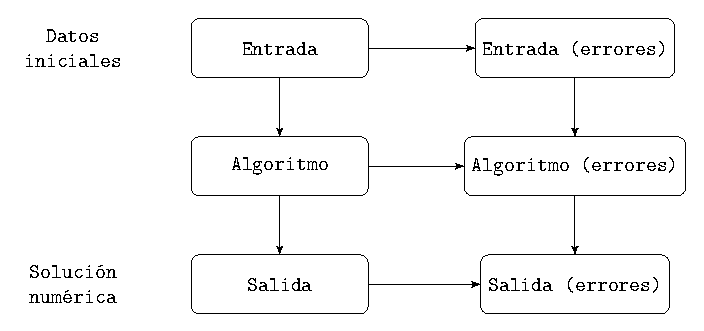
\includegraphics[scale=0.7]{Imagenes/dibujometodonum.eps} 
\end{figure}
\end{frame}
\begin{frame}
\frametitle{La solución que se obtiene}
La solución obtenida por un método numérico es \textocolor{brown(web)}{aproximada}, es decir, hay cierta diferencia entre la solución exacta y la solución numérica.
\\
\bigskip
\pause
Hay que considerar que en ocasiones, no tendremos conocimiento de antemano de la solución \enquote{exacta}.
\end{frame}
\begin{frame}
\frametitle{Principales causas de la diferencia}
\begin{itemize}[<+->]
\item[\ding{217}] Falta de correspondencia entre el problema (modelo) matemático y el fenómeno físico real.
\item[\ding{217}] Errores en los datos iniciales (parámetros de entrada).
\item[\ding{217}] Errores en el método numérico usado para resolver el problema.
\item[\ding{217}] Errores de redondeo en las operaciones aritméticas.
\end{itemize}
\end{frame}
\begin{frame}[fragile]
\frametitle{Nuestra tarea al momento de resolver}
Si tenemos identificadas las posibles fuentes de error, nuestra tarea será minimizar los errores al momento de proponer una solución numérica.
\\
\bigskip
\pause
Veremos la importancia de medir la magnitud de un error.
\end{frame}
% % \subsection{Modelos y métodos numéricos}
% % %\section{\texorpdfstring{this is a very long title I \\ want to}{want to break manually}}
% \begin{frame}
% \frametitle{Conceptos en métodos numéricos}
% Ahora presentaremos los principales conceptos relacionados en métodos numéricos aplicados:
% \pause
% \begin{itemize}[<+->]
% \item Aproximación.
% \item Estabilidad.
% \item Convergencia.
% \end{itemize}
% \end{frame}

\subsection{Aproximación}

\begin{frame}
\frametitle{Aproximación}
Es la proximidad de un modelo numérico al modelo original (diferencial, integral, etc.) o el
grado de aproximación, caracteriza el error que se introduce al hacer discreto el modelo
continuo.
\\
\bigskip
\pause
El grado de aproximación $n$ se estima mediante un factor que tiene el error entre dos modelos.
\end{frame}

\subsection{Estabilidad}

\begin{frame}
\frametitle{Estabilidad}
\begin{itemize}[<+->]
\item[\ding{221}] Caracteriza la manera de propagación de los errores iniciales dentro del algoritmo en el
proceso del cálculo.
\item[\ding{221}] Si el incremento de errores iniciales es considerable y sin ningún control, entonces el
método numérico se llama \textocolor{burgundy}{inestable}.
\item[\ding{221}] Si los errores de cálculos dependen continuamente de los errores iniciales, entonces el método se llama \textocolor{cinnabar}{estable}.
\end{itemize}
\end{frame}
\begin{frame}
\frametitle{Primer ejemplo}
Considera la siguiente sucesión:
\pause
\begin{align*}
\dfrac{1}{3^{n}} \hspace{1cm} n = 0, 1, 2, \ldots
\end{align*}
\pause
Haciendo algunas operaciones sencillas, tenemos los primeros valores de la sucesión de $n = 0$ a $n = 3$:
\pause
\begin{eqnarray*}
( x_{0}, x_{1}, x_{2}, x_{3}, \ldots ) \\[0.5em] \pause
( 1, \, \dfrac{1}{3}, \, \dfrac{1}{27}, \, \dfrac{1}{81}, \ldots )
\end{eqnarray*}
\end{frame}
\begin{frame}
\frametitle{El enésimo más un valor de la sucesión}
Se puede demostrar fácilmente que el enésimo más un término de la sucesión es:
\pause
\begin{align*}
x_{n+1} = \dfrac{13}{3} \, x_{n} - \dfrac{4}{3} \, x_{n-1} \hspace{1cm} n \geq 1
\end{align*}
\pause
También sabemos que se cumple:
\pause
\begin{align*}
\lim_{n \to \infty} \dfrac{1}{3^{n}} = 0
\end{align*}
\end{frame}
\begin{frame}
\frametitle{Pasando a un código}
Elaboremos un código en Jupyter para que nos devuelve los valores de la sucesión.
\\
\bigskip
\pause
Como valores iniciales tomaremos: $x_{0} = 1$ y $x_{1} = \dfrac{1}{3}$, veremos que será muy conveniente usar una lista para almacenar los nuevos valores.
\end{frame}
\begin{frame}[fragile]
\frametitle{Pasando a un código}
\begin{lstlisting}[caption=Implementando el código de la sucesión]
x = [1, 1/3]

print('iteracion \t valor')
print('-'*25)

for i in range(1, 7): |\pause|
	y = (13/3) * x[-1] - (4/3) * x[-2] |\pause|
	x.append(y) |\pause|
	print(i, x[-1], sep='\t\t') 
\end{lstlisting}
\end{frame}
% \begin{frame}
% \frametitle{¿Qué es lo que pasa?}
% Encontramos que los valores obtenidos no son los esperados.
% \\
% \bigskip
% \pause
% ¿Por qué?
% \end{frame}


% \begin{frame}
% \frametitle{El arreglo luego de los cálculos}
% Tendremos entonces que el arreglo con los valores de la sucesión luego de las operaciones es:
% \\
% \pause
% \begin{align*}
% {}&[1,	0.3333333333333333, 3.8888888888888884, \\
% {}&-3.74074074074074, 21.8395061728395, \\
% {}&-45.32921810699587, 155.07681755829896, \\
% {}&-403.195701874714]
% \end{align*}
% \end{frame}
% \begin{frame}
% \frametitle{¿Qué ocurre?}
% Lo que pasa es que el error incluido en el enésimo término $x_{n} + \delta_{n}$ es multiplicado por $13/3$, \pause en cada iteración los errores aumentan poco más de cuatro veces.
% \end{frame}
\begin{frame}
\frametitle{Segundo ejemplo}
Ahora considera la siguiente sucesión:
\pause
\begin{eqnarray*}
\begin{aligned}
y_{n} &= \scaleint{6ex}_{\bs 0}^{1} x^{n} \, e^{x} \dd{x} = \\[0.5em] \pause
&= \dfrac{e}{n+1} - \scaleint{6ex}_{\bs 0}^{1} e^{x} \, \dfrac{x^{n+1}}{n + 1} \dd{x} \\[0.5em] \pause
&= \dfrac{1}{n+1} \big( e - y_{n+1} \big)
\end{aligned}
\end{eqnarray*}
\end{frame}
\begin{frame}
\frametitle{Despejando $y_{n+1}$}
De la expresión anterior, despejamos $y_{n+1}$ y vemos que es necesario ocupar el valor previo: $y_{n}$:
\pause
\begin{align*}
y_{n+1} = \exp - (n + 1) \, y_{n}
\end{align*}
De la integración para $n = 0$, tenemos que $y_{0} = \exp - 1$.
\end{frame}
\begin{frame}
\frametitle{Apoyándose con una gráfica}
En una primera instancia, conforme el valor de $n$ aumenta, la integral (vista como el área debajo de la curva) debería tender a cero.
\\
\bigskip
\pause
Para revisar esto, hagamos una gráfica de $y_{n}$, para $n = 1, 2, 4, 8$.
\end{frame}
\begin{frame}
\frametitle{Gráfica de la función}
\begin{figure}
	\centering
	\includegraphics[scale=0.6]{Imagenes/Estabilidad_02.eps}
\end{figure}
\end{frame}
\begin{frame}
\frametitle{Ejercicio de clase}
\textbf{Ejercicio de clase 2:} Elabora un código y genera la gráfica correspondiente para la función $f(x)$ para $n = 1, 2, 4, 8$.
\\
\bigskip
\pause
Fecha de entrega: para el viernes 1 de septiembre a más tardar 6 pm, vía Moodle.
\end{frame}
% \begin{frame}[allowframebreaks, fragile]
% \frametitle{Gráfica de $y_{n}$}
% import matplotlib.pyplot as plt
% import numpy as np

% def funcion(n, x):
%     return (x**n) * np.exp(x)

% x = np.linspace(0, 1, 100)

% n = [1, 2, 4, 8]

% for i in n:
%     plt.plot(x, funcion(i, x), label='n = {0:}'.format(i))

% plt.title('Grafica de la funcion')
% plt.xlabel('x')
% plt.ylabel('f(x)')
% plt.legend(loc='best')
% plt.show()
% \end{frame}
\begin{frame}
\frametitle{Pasemos al código}
Comprobamos que al menos en la gráfica el límite de la función cuando $n$ aumenta, tiende a cero.
\\
\bigskip
\pause
Ahora pasemos al código.
\end{frame}
\begin{frame}[fragile]
\frametitle{Pasemos al código}
\begin{lstlisting}[caption=Código para el ejemplo 2]
x = [np.exp(1) - 1]

print('iteracion \t valor')
print('-'*25)

for i in range(1, 7): |\pause|
	y = np.exp(1) - (i + 1) * x[-1] |\pause|
	x.append(y) |\pause|
	print(i, x[-1], sep='\t\t')
\end{lstlisting}
\end{frame}
\begin{frame}
\frametitle{¿Dónde está el error?}
Encontramos que la sucesión diverge, ¿pero por qué?
\\
\bigskip
\pause
En cada paso el error $h_{n}$ se multiplica por un número cada vez más grande ($n$), por lo que tenemos estos valores.
\end{frame}
\begin{frame}
\frametitle{Del segundo ejemplo}
Los cálculos efectuados en el segundo ejercicios son \textocolor{red}{inestables}, \pause ya que los errores producidos en una iteración, se incrementan en iteraciones posteriores.
\end{frame}


% % % \begin{frame}
% % % \frametitle{Error de truncamiento}
% % % Se originan al emplear al número finito de términos para calcular un valor que requiere un número infinito de términos.
% % % \\
% % % \bigskip
% % % Por ejemplo, una expresión que permite determinar de forma exacta el valor del número de Euler (base de los logaritmos naturales) a través de una serie de MacLaurin es:
% % % \[ e^{x} = \sum \dfrac{x_{i}}{i!}\]
% % % \end{frame}
% % % \begin{frame}
% % % Sin embargo, una aproximación a dicho valor, puede obtenerse a través de su expresión finita:
% % % \[ e^{x} \simeq \sum_{i=0}^{k} \dfrac{x_{i}}{i!} \hspace{1cm} k<\infty \]
% % % Es claro que esta expresión finita es manejable computacionalmente hablando, al contrario que la fórmula expresada en su forma infinita.
% % % \end{frame}
% % % \begin{frame}
% % % \frametitle{Error por redondeo}
% % % Se origina por el hecho de que una computadora sólo puede representar un número finito de
% % % términos. Para expresar una cantidad con un desarrollo decimal infinito, se tiene que prescindir de la mayoría de ellos.
% % % \\
% % % \bigskip
% % % Por ejemplo, el número $\pi = 3.14159265 \ldots$, tiene un desarrollo decimal infinito no periódico. Por lo tanto, para fines de cálculo, sólo se toman algunos de sus dígitos.
% % % \end{frame}
% % % \begin{frame}
% % % \frametitle{Estrategias}
% % % \begin{itemize}[<+->]
% % % \item \textcolor{blue}{Redondeo}. Prescinde de cierto número de cifras significativas y realiza un ajuste, sobre la última cifra no descartada: $\pi = 3.1416$
% % % \item \textcolor{red}{Corte o poda}: Prescinde de cierto número de cifras significativas sin realizar un ajuste sobre la última cifra no descartada: $\pi = 3.1415$
% % % \end{itemize}
% % % \end{frame}
% \section{Tipos de errores}
% \frame{\tableofcontents[currentsection, hideothersubsections]}
% \subsection{Errores en programación}
% \begin{frame}
% \frametitle{Los errores}
% Como ya hemos mencionado que un programa numérico ejecutado en la computadora, nos va a devolver un resultado que es una aproximación, entonces hay que considerar que existe un \textcolor{red}{error} debido al proceso.
% \end{frame}
% \begin{frame}
% \frametitle{Los errores}
% En métodos numéricos es importante identificar el tipo de error que se obtiene, ya que nos permitirá entonces establecer no sólo un valor, sino la magnitud del error comparada con el valor esperado o \enquote{exacto}.
% \end{frame}
% \begin{frame}
% \frametitle{Nuevos conceptos}
% El error entendido como la suma o consecuencia por un truncamiento o redondeo, se clasifica en:
% \begin{itemize}[<+->]
% \item \textcolor{red}{Error absoluto verdadero}.
% \item \textcolor{orange}{Error relativo verdadero}.
% \item \textcolor{blue}{Error relativo aproximado}.
% \end{itemize}
% \end{frame}
% \subsection{Error absoluto verdadero}
% \begin{frame}
% \frametitle{Error absoluto verdadero}
% Supóngase que $\widehat{p}$ es una aproximación a p.
% \\
% \bigskip
% El error absoluto verdadero se define con la siguiente expresión:
% \[ E_{v} = \vert p - \widehat{p} \vert \]
% Esta definición de error, lo cuantifica en términos brutos.
% \end{frame}
% \begin{frame}
% \frametitle{Tamaño del error}
%  No obstante, una medida que puede describir con mayor detalle o proporción el error, es aquella que lo expresa en términos porcentuales.
%  \\
%  \bigskip
%  Para ello se emplea el error verdadero relativo.
% \end{frame}
% \subsection{Error relativo verdadero}
% \begin{frame}
% \frametitle{Error relativo verdadero}
% Supóngase que $\widehat{p}$ es una aproximación a p. El error relativo verdadero se calcula con la siguiente expresión:
% \[ e_{v} = \dfrac{\vert p - \widehat{p} \vert }{p}\]
% El resultado suele expresarse en términos porcentuales.
% \end{frame}
% \subsection{Error relativo aproximado}
% \begin{frame}
% \frametitle{Error relativo aproximado}
% El error relativo aproximado, mide el error de un método numérico, determinando el error de la iteración actual respecto el error surgido en la iteración anterior:
% \[ e_{a} = \dfrac{\vert \widehat{x}_{i} - \widehat{x}_{i-1} \vert}{\widehat{x}_{i}}\]
% Donde $x_{i}$ es la aproximación actual a $x$ y 
% $x_{i-1}$ es la aproximación anterior a $x$.
% \end{frame}

\subsection{Tolerancia}

\begin{frame}
\frametitle{Tolerancia}
En métodos numéricos suele establecerse una \textocolor{cobalt}{tolerancia} como criterio de paro, \pause tal
que el error relativo aproximado de un método, no exceda dicha tolerancia.
\begin{align*}
E_{\text{rel}} < t
\end{align*}
donde $t$, es tolerancia fijada de antemano.
\end{frame}
\begin{frame}
\frametitle{Tolerancia}
A \textocolor{coquelicot}{menor tolerancia} se tiene \textocolor{cordovan}{mayor precisión} en la aproximación al valor verdadero, \pause sin embargo esto implica un \textocolor{crimsonglory}{aumento en el número de iteraciones} requeridas para detener el método.
\end{frame}

\section{Contaminación en los cálculos}
\frame[allowframebreaks]{\tableofcontents[currentsection, hideothersubsections]}
\subsection{Contaminación en las cuentas}

\begin{frame}
\frametitle{Contaminación en los cálculos.}
Un error en un cálculo numérico \enquote{contamina} las sucesivas evaluaciones.
\\
\bigskip
\pause
Esta propagación puede describirse en términos de dos conceptos relacionados: los de \textocolor{darkbrown}{estabilidad} y \textocolor{darkcerulean}{condición}.
\end{frame}

\subsection{Condición}

\begin{frame}
\frametitle{Condición}
La condición de una función $f (x)$ mide la sensibilidad de los valores de $f (x)$ a pequeños cambios de $x$, se define como:
\pause
\begin{align*}
C = \abs{ \dfrac{E_{\text{rel}} (f (x))}{E_{\text{rel}} (x)} } 
\end{align*}
\end{frame}
\begin{frame}
\frametitle{Definición de condición}
Del teorema del valor medio en cálculo, podemos expresar:
\pause
\begin{align*}
f (x_{T}) - f (x_{A}) & \approx \pderivada{f} (x_{T})(x_{T} - x_{A}) \rightarrow E_{\text{rel}}(f (x)) \approx \\[0.5em] 
 & \approx \dfrac{ \pderivada{f} (x_{T})}{f (x_{T})} (x_{T} - x_{A})
\end{align*}
donde $f (x_{T})$ es el valor exacto de la función, y $f (x_{A})$ es el valor aproximado de la función.
\end{frame}
\begin{frame}
\frametitle{Definición de condición}
Por lo que podemos reescribir el número de condición como:
\pause
\begin{align*}
C \approx \abs{ x_{T} \dfrac{\pderivada{f} (x_{T})}{f (x_{T})} }
\end{align*}
\end{frame}
\begin{frame}
\frametitle{Definición de condición}
Se utilizará ésta definición como definición de condición para funciones $f (x)$ de una variable real.
\\
\bigskip
Entonces el número de condición será:
\pause
\begin{align*}
C = \abs{ x \, \dfrac{\pderivada{f} (x)}{f(x)} }
\end{align*}
\end{frame}
\begin{frame}
\frametitle{Definición de condición}
\begin{align*}
C = \abs{ x \, \dfrac{\pderivada{f} (x)}{f(x)} }
\end{align*}
\setbeamercolor{item projected}{bg=black,fg=white}
\setbeamertemplate{enumerate items}{%
\usebeamercolor[bg]{item projected}%
\raisebox{1.5pt}{\colorbox{bg}{\color{fg}\footnotesize\insertenumlabel}}%
}
\begin{enumerate}[<+->]
\item Para un $x$ dado $0 < C (x) < 1$ se dirá que el problema está bien condicionado, y cuanto menor sea $C$, mejor condicionado.
\item Si $C (x) > 1$, el problema estará mal condicionado.
\item Si $C (x) = 1$, el error relativo se mantiene.
\end{enumerate}
\end{frame}
\begin{frame}
\frametitle{Ejemplos}
Las siguientes funciones están bien condicionadas?
\pause
\setbeamercolor{item projected}{bg=cobalt,fg=white}
\setbeamertemplate{enumerate items}{%
\usebeamercolor[bg]{item projected}%
\raisebox{1.5pt}{\colorbox{bg}{\color{fg}\footnotesize\insertenumlabel}}%
}
\begin{enumerate}[<+->]
\item $f (x) = \sqrt{x} \hspace{1.5cm} C (x) = ?$
\item $g (x) = x^{2}-1 \hspace{1.5cm} C (x) = ?$
\end{enumerate}
\end{frame}

\subsection{Nuevamente la estabilidad}

\begin{frame}
\frametitle{Estabilidad}
Ya revisamos que la estabilidad de un algoritmo describe la sensibilidad de un método numérico específico
respecto a los inevitables errores de redondeo cometidos durante su ejecución en aritmética de precisión finita.
\end{frame}
\begin{frame}
\frametitle{Revisando la estabilidad}
Consideremos la siguiente función:
\begin{align*}
f (x) = \sqrt{x + 1} - \sqrt{x}
\end{align*}
\pause
Su número de condición es:
\pause
\begin{align*}
C (x) = \abs{ x \, \dfrac{\pderivada{f} (x)}{f(x)} } = \dfrac{x}{2 \, \sqrt{x} \sqrt{x+1}}
\end{align*}
\pause
Vemos que $C (x) < \dfrac{1}{2}$ para $x > 0$, por lo que la función está bien condicionada pero ...
\end{frame}
\begin{frame}
\frametitle{Revisando la estabilidad}
El pseudocódigo para calcular $x$ de tal forma que se vayan realizando las operaciones, es:
\pause
\setbeamercolor{item projected}{bg=apricot,fg=black}
\setbeamertemplate{enumerate items}{%
\usebeamercolor[bg]{item projected}%
\raisebox{1.5pt}{\colorbox{bg}{\color{fg}\footnotesize\insertenumlabel}}%
}
\begin{enumerate}[<+->]
\item obtener $x$
\item $y = x + 1$
\item $f = \text{sqrt } (y)$
\item $g = \text{sqrt } (x)$
\item $h = f - g$
\end{enumerate}
\end{frame}
\begin{frame}
\frametitle{Revisando la estabilidad}	
El procedimiento \textocolor{bole}{es inestable} para valores grandes de $x$, dado el paso 5, por lo que debemos de reestructurar la función.
\end{frame}

\subsection{Eficiencia}

\begin{frame}
\frametitle{Eficiencia}
\emph{Debemos evitar que todo algoritmo sea inestable}. 
\\
\bigskip
Si existieran varios métodos para evaluar una misma función, entonces conviene utilizar aquel que sea más eficiente, \pause es decir, \textocolor{byzantium}{el más rápido}.
\end{frame}
\begin{frame}
\frametitle{Eficiencia}
\textocolor{blue}{Hay que aprovechar al máximo los recursos: hardware, software, algoritmos, para resolver problemas más complejos y no para resolver peor problemas simples.}
\end{frame}
\begin{frame}
\frametitle{Cita oportuna}
\begin{quote}
Cualquiera puede escribir código que una máquina entiende. Los buenos programadores escriben código que los humanos pueden entender.
\end{quote}
Martin Fowler.
\end{frame}
\begin{frame}
\frametitle{Ejemplo de eficiencia}
Por ejemplo, para calcular $x**4$ para un $x$ dado, no es buena idea calcular $x**4.0$ (exponente en punto flotante).
\\
\bigskip
\pause
La mejor idea consiste en economizar el cálculo en dos pasos:
\begin{align*}
x2 &= x*x \\
x4 &= x2*x2
\end{align*}
\pause
y no un producto de la forma:
\begin{align*}
x4 = x*x*x*x
\end{align*}
\end{frame}
\begin{frame}
\frametitle{Ejemplo: Evaluación de polinomios}
Supongamos que queremos evaluar el polinomio:
\pause
\begin{align*}
P (x) = 2 + 4 \, x - 5\, x^{2} + 2\,  x^{3} - 6 \, x^{4} + 8 \, x^{5} + 10 \, x^{6}
\end{align*}
\pause
Contando con que cada potencia de exponente $k$ entero como $k-1$ productos, tendríamos que el total de productos para evaluar en forma directa es:
\[ 1+2+3+4+5+6=21\]
Además de seis sumas.
\end{frame}
\begin{frame}
\frametitle{Ejemplo: Evaluación de polinomios}
Una mejora en el algoritmo , es calcular primero las potencias de forma sucesiva:
\begin{align*}
x^{2} & = x*x \\
x^{3} & = x*x^{2} \\
x^{4} & = x*x^{3} \\
x^{5} & = x*x^{4} \\
x^{6} & = x*x^{5}
\end{align*}
\end{frame}
\begin{frame}
\frametitle{Ejemplo: Evaluación de polinomios}
De tal forma que se añade un producto por cada potencia, para un total de productos:
\begin{align*}
1 + 2 + 2 + 2 + 2 + 2 = 11
\end{align*}
\end{frame}
\begin{frame}
\frametitle{Ejemplo: Evaluación de polinomios}
Con el polinomio:
\begin{align*}
P (x) = 2 + 4 \, x - 5 \,  x^{2} + 2 \, x^{3} - 6 \, x^{4} + 8 \,  x^{5} + 10 \, x^{6}
\end{align*}
\pause
podemos mejorar el algoritmo de la siguiente manera:
\pause
\fontsize{12}{12}\selectfont
\begin{align*}
P (x) = 2 + x \left\lbrace 4 + x \left( -5 + x \left[ 2 + x \left(-6 +x \left\lbrace 8+x*10 \right\rbrace \right) \right] \right) \right\rbrace 
\end{align*}
\end{frame}
\begin{frame}
\frametitle{Ejemplo: Evaluación de polinomios}
Para evaluar un polinomio de grado $n$ en el que ninguno de los coeficientes es cero, se necesitan
\\
\medskip
\pause
\begin{tabular}{l l}
$\dfrac{n\ , (n + 1)}{2}$ & Productos para el primer método \\
$2\ , n - 1$ & para el segundo métodos \\
$n$ & para el tercero
\end{tabular}
\\
\medskip
\pause
Antes de escribir una línea de código, hay que revisar la manera en que podemos optimizar la solución del problema.
\end{frame}

\section{Algoritmo de Horner}
\frame{\tableofcontents[currentsection, hideothersubsections]}
\subsection{Construyendo el algoritmo}

\begin{frame}
\frametitle{Algoritmo de Horner}
Dado el polinomio:
\begin{align*}
P (x) = a_{0} + a_{1} \, x + \ldots + a_{n} \, x^{n} \hspace{1cm} a_{n} \neq 0
\end{align*}
\pause
La evaluación de $P (x)$ para cierto valor de $x = z$ se puede realizar en $n$ pasos mediante el siguiente procedimiento:
\end{frame}
\begin{frame}
\frametitle{Algoritmo de Horner}
\begin{eqnarray*}
\begin{aligned}
b_{n} &= a_{n} \\ \pause
b_{n-1} &= a_{n-1} + z*b_{n} \\ \pause
b_{n-2} &= a_{n-2} + z*b_{n-1} \\ \pause
\vdots \\
b_{0} &= a_{0} + z*b_{1}
\end{aligned}
\end{eqnarray*}
\end{frame}
\begin{frame}
\frametitle{Pseudocódigo}
\setbeamercolor{item projected}{bg=copper,fg=white}
\setbeamertemplate{enumerate items}{%
\usebeamercolor[bg]{item projected}%
\raisebox{1.5pt}{\colorbox{bg}{\color{fg}\footnotesize\insertenumlabel}}%
}
\begin{enumerate}[<+->]
\item $b_{n} = a_{n}$
\item repetir mientras $n > 0$
\item $n = n - 1$
\item $b = a_{n} + z*b$
\item volver al paso 2
\item $p (z) = b$
\end{enumerate}
\end{frame}
\begin{frame}
\frametitle{Ejercicio: evalúa el polinomio $P(x)$}
\begin{align*}
P (x) =2 + 4 \, x - 5 \, x^{2} + 2 \, x^{3} - 6 \, x^{4} + 8 \, x^{5} + 10 \, x^{6}
\end{align*}
\\
\bigskip
\pause
Para simplificar el resultado, nos apoyaremos con una tabla con el valor $x$ a evaluar y $P (x)$ el valor obtenido:
\end{frame}
\begin{frame}
\frametitle{Ejercicio: evalúa el polinomio $P(x)$}
\begin{table}
\centering
\begin{tabular}{S | c}
$x$ & $P (x)$ \\
\hline -1.5 & \\
\hline -0.65 & \\
\hline 0.1 & \\
\hline 1.4 & \\
\hline 2.87 & 
\end{tabular}
\end{table}
\end{frame}
\begin{frame}
\frametitle{Resultado}
El polinomio $P(x)$ evaluado con el método de Horner:
\\
\medskip
\renewcommand{\arraystretch}{1}
\begin{table}
\centering
\begin{tabular}{c | c }
$x$ & $P (x)$ \\
\hline $-1.5$ & $0.78125$ \\
\hline $-0.65$ & $-4.50683$ \\
\hline $0.1$ & $2.35149$ \\
\hline $1.4$ & $98.55968$ \\
\hline $2.87$ & $6758.70245$ \\
\end{tabular}
\end{table}
\end{frame}
\begin{frame}[fragile]
\frametitle{La primera respuesta}
Podemos responder el ejercicio con una propuesta de evaluación directa, como se presenta en el siguiente código:
\end{frame}
\begin{frame}[allowframebreaks,fragile]
\frametitle{Código de primera respuesta}
\begin{lstlisting}[caption=Código directo]
def eval_polinomio(x):
    valor = 2 + 4 * x - 5 * x**2 + 2 * x**3 - 6 * x**4 + 8 * x**5 + 10 * x**6
    return valor

x0 = [-1.5, -0.65, 0.1, 1.4, 2.87]

print('x0 \t Evaluacion')
print('-'*20)

for i in x0:
    resultado = eval_polinomio(i)
    print('{0:}  \t {1:.6f}'.format(i, resultado))
\end{lstlisting}
\end{frame}

\begin{frame}
\frametitle{Extendiendo la respuesta al problema}
¿Cómo resolvemos el problema usando una función para el método de Horner? \pause

¿Presentamos una tabla con formato de salida? \pause

¿Graficamos $P (x)$ y un conjunto de datos evaluados? \pause

¿Evaluamos el error relativo?
\end{frame}
\begin{frame}
\frametitle{Extendiendo la respuesta al problema}
Ya contamos con las herramientas necesarias para extender la respuesta al problema, \pause en nuestro código podemos agregar funciones, \pause ajustar formatos de salida en los resultados, \pause graficar el polinomio y los puntos (o un conjunto diferente de puntos), \pause y obtener el error relativo.
\end{frame}
\begin{frame}
\frametitle{Pasos a resolver}
\setbeamercolor{item projected}{bg=cyan,fg=black}
\setbeamertemplate{enumerate items}{%
\usebeamercolor[bg]{item projected}%
\raisebox{1.5pt}{\colorbox{bg}{\color{fg}\footnotesize\insertenumlabel}}%
}
\begin{enumerate}[<+->]
\item Conviene definir una función que resuelva la evaluación del método de Horner.
\item Para obtener el error relativo, se debe de evaluar el polinomio y considerar que los valores obtenidos, son los valores exactos.
\item Comparamos los resultados mediante una gráfica que represente los dos resultados de la evaluación.
\end{enumerate}
\end{frame}
\begin{frame}[fragile]
\frametitle{Estructuramos el código en \python.}
Ocuparemos dos listas para:
\setbeamercolor{item projected}{bg=darkpastelgreen,fg=black}
\setbeamertemplate{enumerate items}{%
\usebeamercolor[bg]{item projected}%
\raisebox{1.5pt}{\colorbox{bg}{\color{fg}\footnotesize\insertenumlabel}}%
}
\begin{enumerate}[<+->]
\item Los valores $z$ donde queremos evaluar el polinomio $P (x)$.
\item Los coeficientes del polinomio $P (x)$.
\end{enumerate}
\end{frame}
\begin{frame}[fragile]
\frametitle{Función de Horner.}
\fontsize{14}{14}\selectfont
\begin{lstlisting}[caption=Código para la función de Horner]
# Metodo de Horner

def P_Horner(a, x):
    P_Hor=0
    for n in range(len(a)-1, -1, -1):     
        P_Hor=a[n] + P_Hor * x
    return P_Hor
\end{lstlisting}
\end{frame}
\begin{frame}[fragile]
\frametitle{Función que evalúa directamente $P(x)$.}
\fontsize{14}{14}\selectfont
\begin{lstlisting}[caption=Evaluación directa de la función]
# Evaluacion directa

def P_Directo(x):
    return 2 + 4*x - 5 * x**2 + 2 * x**3 -6 * x**4 + 8 * x**5 + 10 * x**6
\end{lstlisting}
\end{frame}
\begin{frame}[fragile]
\frametitle{Calculamos el error relativo.}
\begin{lstlisting}[caption=Evaluación del error relativo]
# Calculo de error relativo

def Err_Rel(pdirecto, pHorner): return (pdirecto - pHorner)/pdirecto * 100
\end{lstlisting}
\end{frame}
\begin{frame}[fragile]
\frametitle{Uso de valores para evaluar}
\begin{lstlisting}[caption=Valores para evaluar]
# Valores de x0 para evaluar P(x0)
x0 = [-1.5, -0.65, 0.1, 1.4, 2.87]

# Coeficientes de P(x)
a = [2,4, -5, 2, -6, 8, 10]
\end{lstlisting}
\end{frame}
\begin{frame}[fragile]
\frametitle{Mostramos el error relativo de los puntos a evaluar.}
\fontsize{14}{14}\selectfont
\begin{lstlisting}[caption=Error relativo calculado]
# Evaluacion de valores de P(x0)

for i in range(len(x0)):
	error_rel = Err_Rel(P_Directo(x0[i]), P_Horner(a, x0[i]))
    print ("P({0:.2f}) = {1:.5f} , Error relativo = {2:}".format(x0[i],P_Horner(x0[i]), error_rel)) 
\end{lstlisting}
\end{frame}
\begin{frame}[fragile]
\frametitle{Completando el código}
Con el código que se ha presentado, podemos obtener en la terminal los valores obtenidos al usar el método de Horner, el valor con la evaluación directa y el error relativo.
\\
\bigskip
\pause
Te pedimos que incorpores una rutina de graficación para mostrar los puntos de la lista $x0$ y el polinomio $P(x)$.
\end{frame}
\begin{frame}[fragile]
\frametitle{Mostrando los resultados}
\begin{figure}
	\centering
	\includegraphics[scale=0.55]{Imagenes/MetodoHorner_01.eps}
\end{figure}
\end{frame}
\begin{frame}[fragile]
\frametitle{Extendiendo la evaluación de puntos}
El siguiente paso será incluir un mayor número de puntos a evaluar con el método de Horner.
\\
\bigskip
\pause
Para no incluir una lista con $50$ puntos distribuidos en el intervalo $(-2, 3)$, usaremos la función $\mbox{linspace}(-2, 3, 50)$ para crear ese conjunto.
\end{frame}
\begin{frame}[fragile]
\frametitle{Resultado gráfico más completo}
En la gráfica se muestra el conjunto de datos que se evalúan con el método de Horner (puntos rojos), así como la función evaluada directamente (en línea continua) se compara, podemos ver que los resultados son prácticamente los mismos.
\end{frame}
\begin{frame}[fragile]
\frametitle{Resultado gráfico más completo}
\begin{figure}
	\centering
	\includegraphics[scale=0.45]{Imagenes/MetodoHorner.eps} 
\end{figure}
\end{frame}
\begin{frame}[allowframebreaks, fragile]
\frametitle{Los resultados en una gráfica.}
\begin{lstlisting}[caption=Elaboración de la gráfica]
import matplotlib.pyplot as plt
import numpy as np

x = np.linspace(-2., 3., 50)

plt.plot(x, P_Horner(a, x),'ro', label='Metodo de Horner')

plt.plot(x, P_Directo(x), label='Evaluacion Polinomio')

plt.title('Comparacion grafica')
plt.legend(loc='upper left')
plt.grid(True)
plt.show()
\end{lstlisting}
\end{frame}
\begin{frame}
\frametitle{Función para generar secuencia de reales}
Ya hemos mencionado que la librería \funcionazul{numpy} extiende el conjunto de funciones matemáticas que se tienen dentro de la otra librería \funcionazul{math}.
\\
\bigskip
\pause
Veamos la sintaxis de la función \funcionazul{linspace} que aparece en la rutina de graficación.
\end{frame}
\begin{frame}
\frametitle{La función \texttt{linspace}}
Sintaxis mínima:
\\
\medskip
\texttt{linspace(inicio, fin, num=50)}
\\
\medskip
Donde:
\begin{itemize}
\item \texttt{inicio}: es el valor a partir del cual queremos generar la secuncia de puntos.
\item \texttt{fin}: es el valor en donde se detiene la secuencia de puntos.
\item \texttt{num}: es el número de puntos que se genera en el intervalo, por defecto se generan 50 puntos.
\end{itemize}
\end{frame}
\begin{frame}
\frametitle{La secuncia que se genera}
Lo que obtenemos con \funcionazul{linspace}, es una secuencia de puntos distribuidos uniformemente en el intervalo \texttt{[inicio, fin]}.
\end{frame}
\end{document}
